\chapter{Implementation}
\label{chap:implementation}

%%%%%%%%%%%%%%%%%%%%%%%%%%%%%%%%%%%%%%%%%%%%%%%%%%%%%%%%%%%%%%%%%%%%%%%%%%%%%%%%%%%%%%%%%%%%%%%%%%%%

This chapter will document the implementation process of the robot control system by going through each subsystem package in turn. The nodes contained in each subsystem will be detailed, elaborating on their general design, published and subscribed topics, configuration, and reasons for their necessity, as well as general commentary. Where appropriate, reasons for choosing particular existing packages over any others will also be discussed. The chapter will finish by briefly describing how these subsystems were integrated to give the complete robot control system as required.

%%%%%%%%%%%%%%%%%%%%%%%%%%%%%%%%%%%%%%%%%%%%%%%%%%%%%%%%%%%%%%%%%%%%%%%%%%%%%%%%%%%%%%%%%%%%%%%%%%%%

\section{Hardware Operation}

The hardware operations subsystem was implemented as a \texttt{hexapod\_hw} package. This subsystem was responsible for interfacing with the physical hardware on-board the robot, providing access to that hardware through ROS topics. Two components were necessary, one which handled broadcasting imagery streams from the RGB-D camera and another for handled servo controller commands, which will be detailed in the following sections.

\subsection{RGB-D Camera Driver}

As RGB-D cameras are commonly used devices in robotics, a standard package for interfacing with them was already available. A wrapper for the \emph{OpenNI2} library is provided by the \texttt{openni2\_camera} \cite{ros_wiki_openni2_camera} and \texttt{openni2\_launch} \cite{ros_wiki_openni2_launch} packages. This provided us with direct access to the imagery from the camera through ROS topics, rather than having to deal with the specifics of the \emph{OpenNI2} library itself. The former package provides a single nodelet which acquires and publishes the image data, whereas the latter package provides a means for starting that nodelet.

This driver publishes image data from the camera on a number of different topics with various data types. Only a subset of these are particularly useful to us, however. The topic \texttt{/camera/rgb/image} provides the general optical feed from the camera, and the topic \texttt{/camera/depth\_registered/image} provides a registered depth feed from the camera, both of message type \texttt{Image}. Registered, in this case means, that the depth image has been aligned to the colour image. An example of the output from these topics is shown in \autoref{fig:rgbd_images1}. While the depth feed can be interpreted as an 8-bit monochrome image for displaying on-screen, the image is actually given in a 16-bit format, where each pixel value represents the distance from the sensor in millimeters. Additionally, the depth data is available in a point cloud format, published on \texttt{/camera/depth/points} as \texttt{PointCloud2} messages. This can be visualised in RViz, an example of which is shown in \autoref{fig:rgbd_images2}. The \texttt{openni2\_launch} package also publishes static \emph{tf} transforms for the individual sensors on the camera, such that the slight differences in perspectives between the sensors can be corrected.

\begin{figure}[!h]
    \centering
    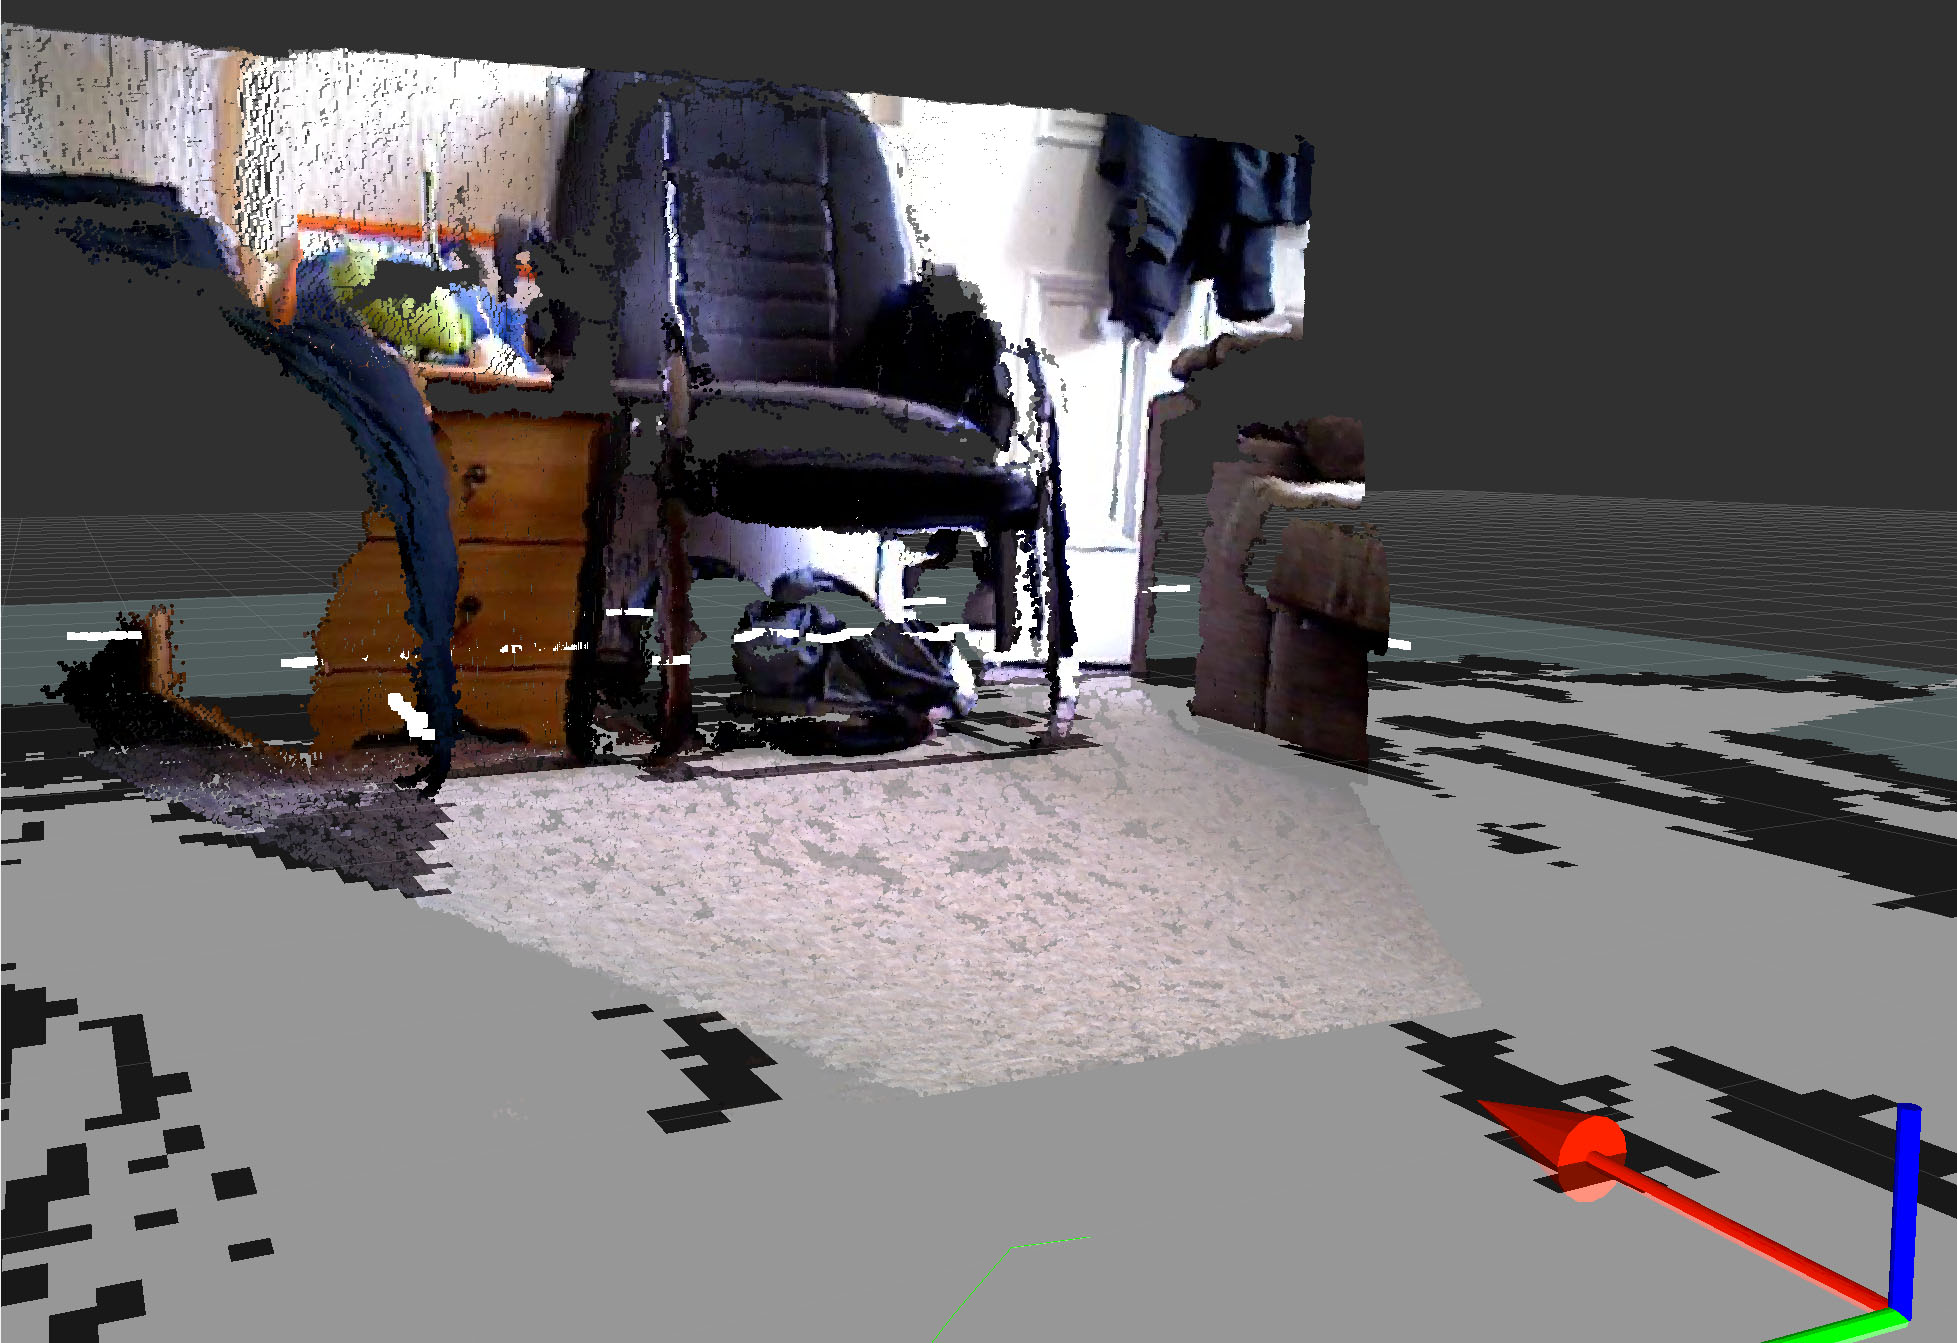
\includegraphics[width=12cm]{rgbd_pc2.jpg}
    \caption{Example point cloud output from the RGB-D camera mounted on top of the robot, as given by the \texttt{openni2\_camera} package, visualized using \emph{rviz}. In this case, the points are projected into 3D space relative to the robot's position, and then coloured using the corresponding pixels on the RGB image.}
    \label{fig:rgbd_images2}
\end{figure}

Understanding these package was rather troublesome as both the wiki and GitHub pages documenting them were (and still are) completely blank. Instead, the documentation for a similar set of these packages for the first version of \emph{OpenNI}, named \texttt{openni\_launch}, was used \cite{ros_wiki_openni_launch}. Regardless, there was little difficulty in integrates this package due the little configuration it requires.

\subsection{Servo Driver}

While there were already drivers available for the RGB-D sensor, this was not the case for the servo controller. A custom \texttt{servo\_controller} node was developed which accepts command messages through a topic. This node then relays commands to the controller by converting them into the format specified in the protocol. Furthermore, the node is implemented in such a way that it can be used to move any number of servos connected to the controller, not just the eighteen as required by the hexapod. By creating this node, we centralise the point at which the control system communicates with the servo controller. This alleviates the need for any other node to understand the underlying protocol and also allows us to swap out the servo controller if need be with one that is completely different, without disrupting any commanding nodes. This also helps with any possible conflicts as commands are serialised at this point---it is not possible for two commands to be sent at the exact time.

The node listens for movement commands on a topic named \texttt{direct} relative to its namespace. By using a topic over a service, we ensure that any node sending commands to the controller need not wait for the command to actually be issued. This simplifies any timing necessities for a commanding node, such as those performing locomotion duties. A custom \texttt{ServoCommand} message had to be created to support this topic as none of the standard messages distributed with ROS were appropriate. In particular, it was necessary that a command include which servo to rotate, the target position, and how long it should take to move to that angle. The specification for this message is shown in \autoref{tab:servocommand_msg}. Having received one of these messages, the node will relay it to the controller after performing the steps necessary to transform it into the required protocol format.

\begin{table}[!h]
	\centering
	\begin{tabular}{ r r p{10cm} }
		\toprule
		\textbf{Name} & 
		\textbf{Type} & 
		\textbf{Description} \\
		\midrule

		\texttt{index} & 
		\texttt{uint8} &
		An index indicating which servo to rotate, where $0 \leq i \leq 31$. \\
		
		\hline

		\texttt{angle} & 
		\texttt{int16} & 
		The target position that the servo should rotate to in degrees, generally where $0 \leq \theta \leq 180$. This can also accept negative values such that it can be used for supplying servo offsets. \\
		
		\hline

		\texttt{duration} &
		\texttt{float32} &
		The duration for how long the rotation should take in seconds, essentially setting a speed for the rotation. \\
		\bottomrule
	\end{tabular}
	\caption{The specification for the \texttt{ServoCommand} message as used by the \texttt{servo\_controller} node. A \texttt{header} field is also included but omitted for brevity.}
	\label{tab:servocommand_msg}
\end{table}

To specify the time taken to rotate the servo, a \texttt{duration} primitive could have been used rather than a \texttt{float32} \cite{ros_wiki_msg}. These primitives are by backed by classes in the client libraries such that they can be manipulated more easily \cite{ros_api_duration_msg}. For example, a \texttt{duration} can be added to a \texttt{time}---another primitive---resulting in a new \texttt{time}. While this may be useful, the duration can only be specified using integers in either \emph{seconds} or \emph{nanoseconds} \cite{ros_api_duration_msg}. This granularity can be quite tedious as the rotation durations are usually specified in the range of hundreds of milliseconds. To give an example, to rotate with a duration of a 0.1 seconds, the duration would need to be specified as either 1 second---thus being wildly inaccurate---or 100,000,000 nanoseconds---a rather excessively large number. It was for this reason that \texttt{float32} was chosen as it allows time to specified in seconds directly with fractions as necessary.

As standard with UNIX systems, the device presents itself as a file located in the \texttt{/dev} directory once connected which can be read from and written to \cite{unix_devices}. In this case, the device shows itself to be an external serial port with path \texttt{/dev/ttyAMC0} though this may vary depending on system configuration. While it is possible to open this file and begin writing directly using standard Python file semantics, a number of settings must be applied beforehand to ensure correct operation. A library named \emph{pySerial} was used to simplify this process by encapsulating access to the serial port while still giving a means of reading and writing using the familiar file semantics \cite{pyserial}. Additionally, this library provides the same interface to the serial port across many platforms allowing the controller node to be used in a variety of situations \cite{pyserial}.

A number of calculations must be performed to convert the supplied \texttt{ServoCommand} message into the right format for the protocol. Firstly, the protocol mandates that servo indices begin from 1, rather than 0. For this, we simply increment the supplied \texttt{index} by 1. Secondly, the target position sent to the controller must be a PWM duration where 1.5\textmu{}s corresponds to 0\textdegree{} and 2.5\textmu{}s corresponds to 180\textdegree{}. As we know the supplied \texttt{angle} will fall between 0 and 180, we can apply formula to get the correct value, specifically $1500 + (\theta / 180 \times 1000)$. Finally, the protocol expects the duration to be an integer representing number of milliseconds. This conversion is achieved by simply multiplying the value by 1000, converting the supplied \texttt{duration} field from seconds to milliseconds.

Due to some quirk in the servo controller's programming, a time delay had to be added between sending commands. Without this, commands would get lost or abort midway through a rotation. A delay of 3 milliseconds was adequate to correct this without causing timing issues elsewhere in the system, minimized purely through trial and error. Seemingly, the controller requires some processing time after a command before it can begin processing another. Unfortunately, it is impossible to diagnose this issue any further as no source code is available, nor does the protocol documentation mention this limitation in any form \cite{torobot_manual}.

%%%%%%%%%%%%%%%%%%%%%%%%%%%%%%%%%%%%%%%%%%%%%%%%%%%%%%%%%%%%%%%%%%%%%%%%%%%%%%%%%%%%%%%%%%%%%%%%%%%%

\section{Locomotion}

The locomotion subsystem was implemented as a \texttt{hexapod\_locomotion} package. This subsystem was responsible for providing the walking motions necessary to move the robot around an environment. Specifically, it was necessary that the subsystem provide a layer of abstraction above these motions, hiding away the complexities of the particular walking gait. Additionally, the subsystem would have to provide a means of calibrating the limbs such that they can be aligned to the correct angles, as well as a means for controlling the robot by manual input---in this case using a gamepad controller. Four components were devised to provide this functionality which will be detailed in the following sections.

\subsection{Limb Controller}

To simplify joint control, a further layer of abstraction atop the \texttt{servo\_controller} node was added. This layer of abstraction divides the servos into logical groupings based on the particular limb and limb section (i.e., foot, shin, body). Without this abstraction, any commanding node would need to calculate the correct servo index based on what limb and which part of the limb it wished to rotate. A custom \texttt{limb\_controller} node was implemented to provide these groupings, taking away the burden of any calculation. Furthermore, angle offsets and inversion flags can be supplied per-servo through this node, providing a means of calibration. This node essentially acts as a proxy for the \texttt{servo\_controller} node, modifying the messages as necessary.

The \texttt{limb\_controller} node listens for \texttt{ServoCommand} messages on three topics relative to itself. These topics are \texttt{/joint/body}, \texttt{/joint/shin}, and \texttt{/joint/foot}, each controlling the body, shin, and foot sections respectively. When a message is received on these topics, a new \texttt{ServoCommand} message is created with correct servo index and any angle adjustments. This is then sent to the \texttt{servo\_controller} node to control the requested limb section proper.

\begin{figure}[!h]
    \centering
    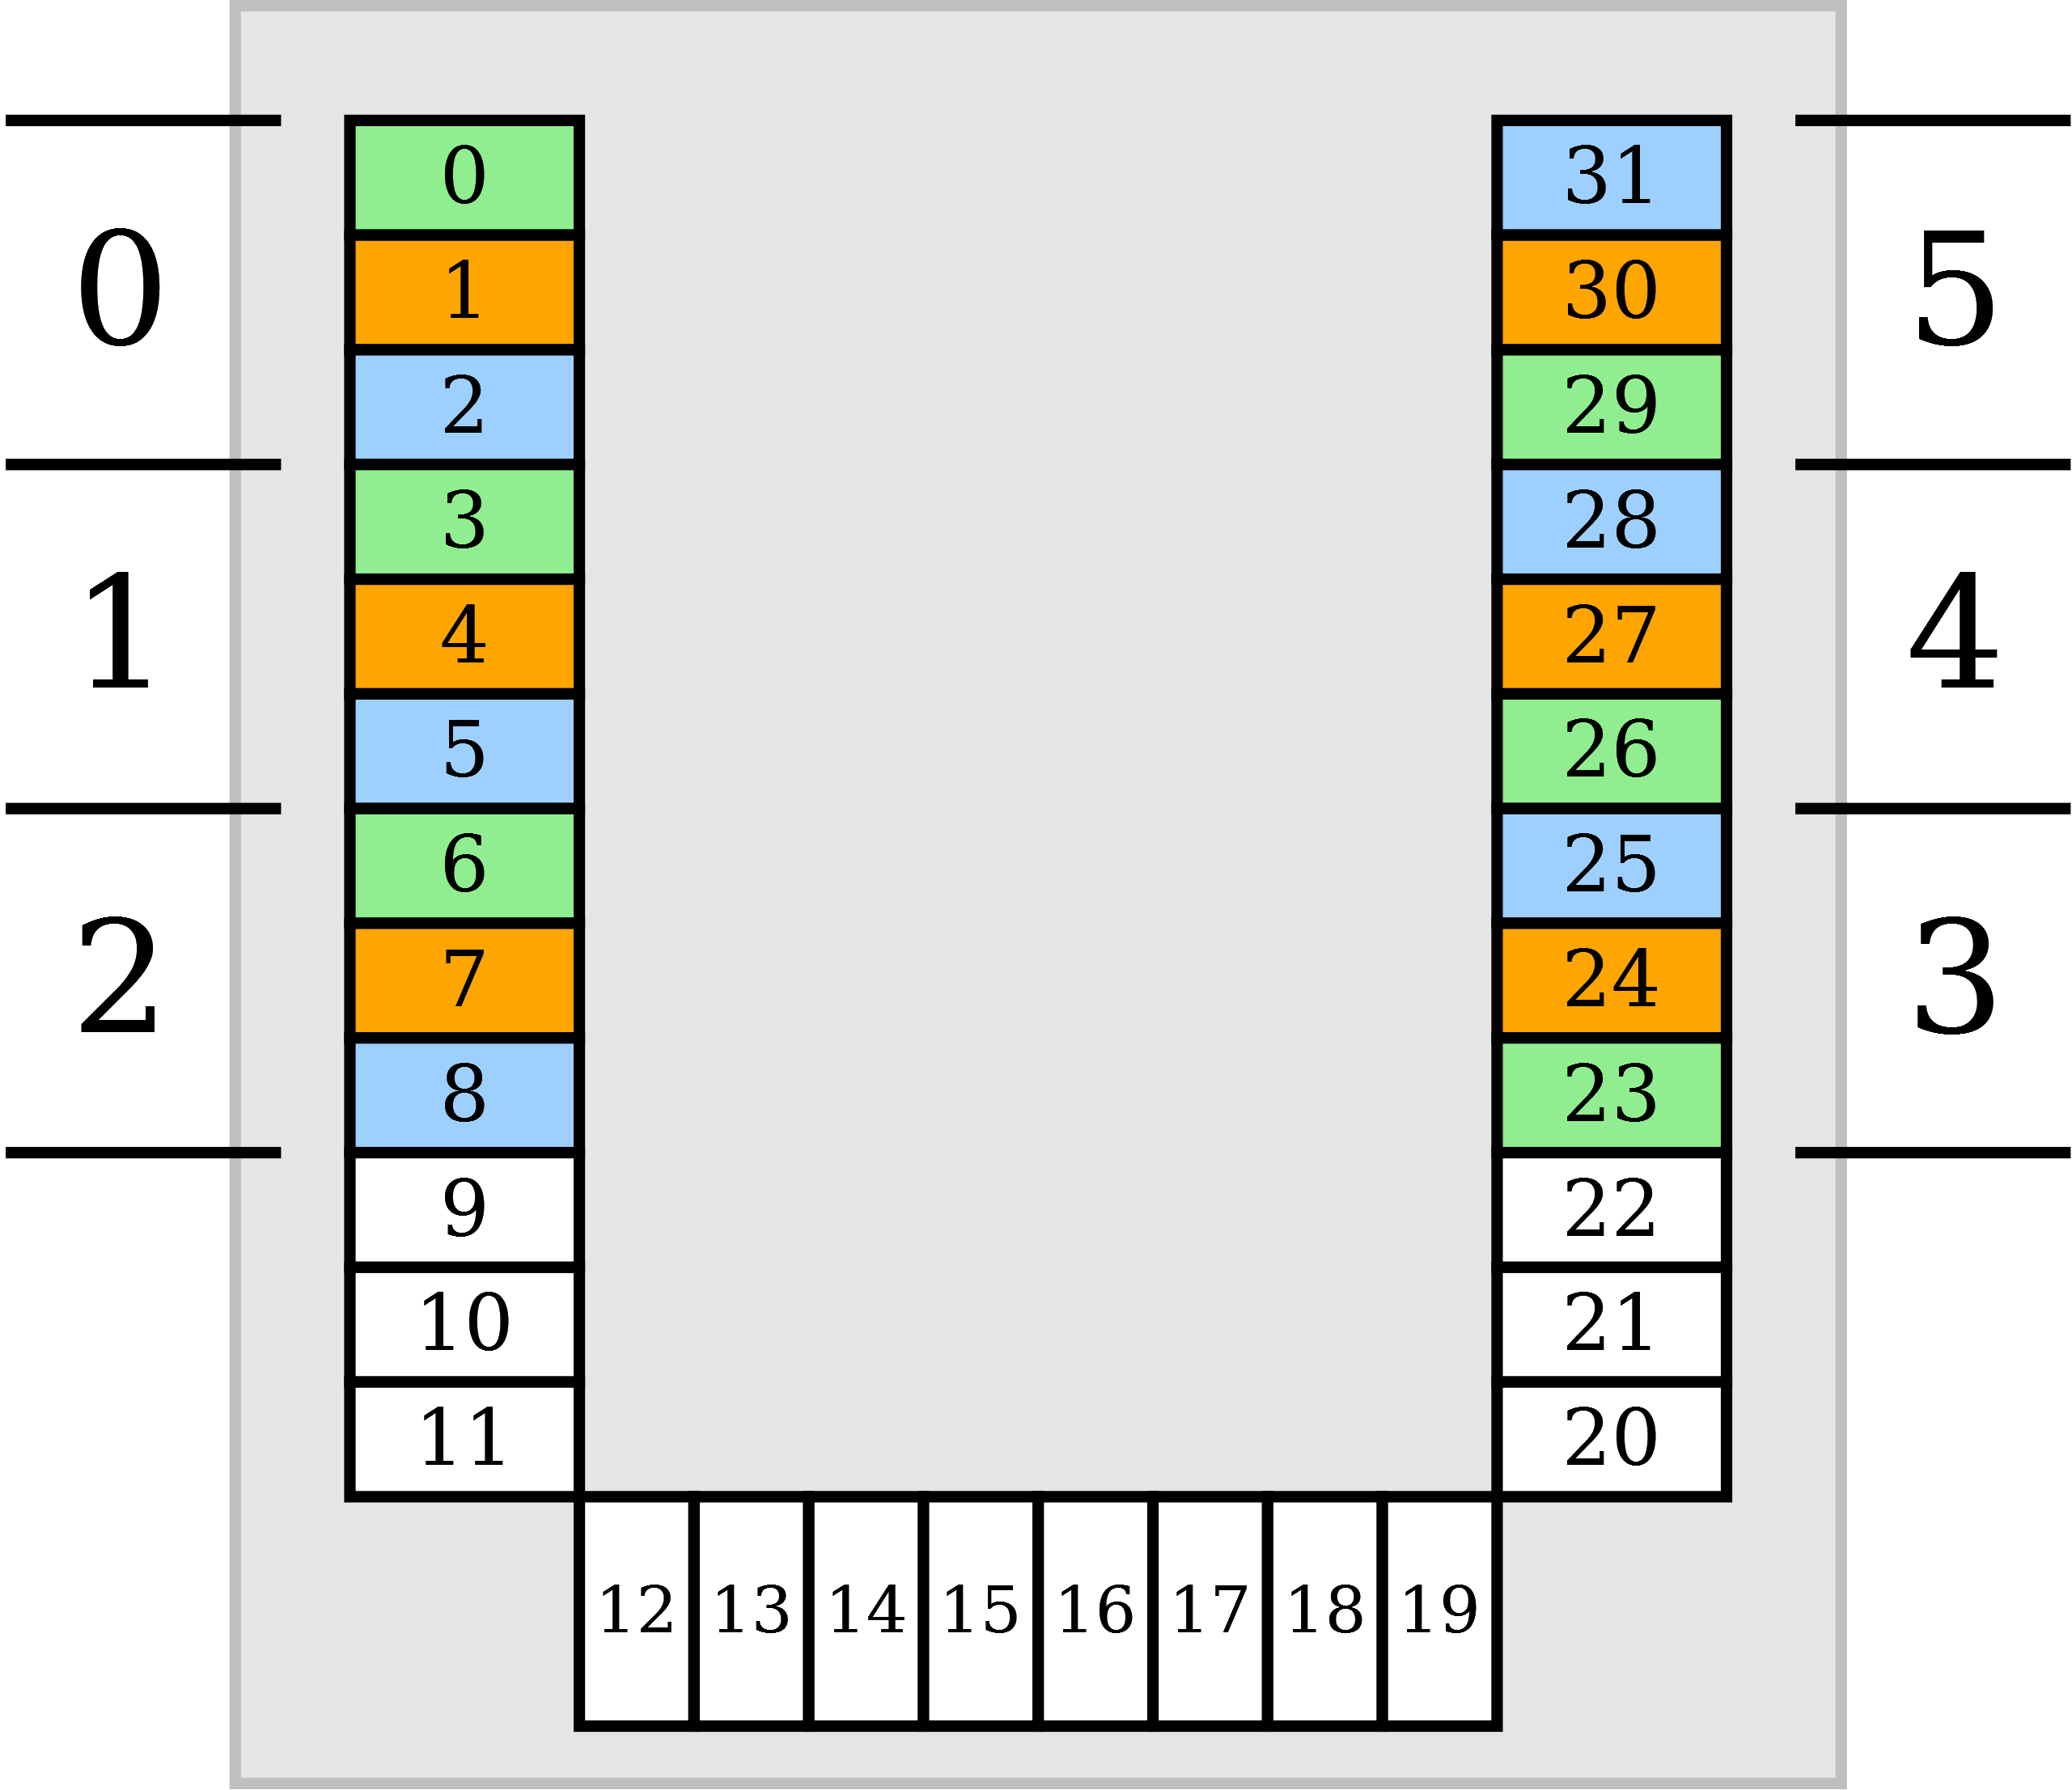
\includegraphics[width=8cm]{limb_controller.png}
    \caption{A simplified diagram showing where each servo on the robot is connected to the servo controller along with their corresponding limb number. Green boxes represent body joint servos, orange boxes represent shin joint servos, and blue boxes represent foot joint servos. White boxes represent unoccupied connections. Connecting the servos in this way allows for better cable management as well as giving the largest amount of cable slack to each limb.}
    \label{fig:servo_pins}
\end{figure}

Some logic and arithmetic must be performed to calculate the correct servo index for a given limb index and limb section. A diagram showing how the servos are connected to the servo controller is shown in \autoref{fig:servo_pins}. From this, it can be seen that servos are grouped per limb and then ordered by particular limb section. For a given limb index $i$, the servo index of the first joint in the grouping---the body joint---can be calculated by the formula $s = i \times 3$. Then, a further displacement can be added to find the servo index of the other joints. To find the servo index of the shin joint we calculate $s = s + 1$, and to find the servo index of foot joint we calculate $s = s + 2$. While these formulae gives the correct indices for the first three limbs, we must also take into account the fact that the remaining three limbs begin at a servo index of 23 rather than 0. A trivial piece of logic to deal with this was added which simply increments the final servo index by 23 should the supplied limb be on that side. A code snippet is shown in \autoref{fig:actual_index} showing the specifics of how this is calculated.

\begin{figure}[!h]
    \centering
	\begin{lstlisting}[language=Python]
	def __actual_index(index, offset):
		actual_index = ((index % 3) * 3) + offset
		if index >= 3:
			actual_index += (31 - 8)

		return actual_index
	\end{lstlisting}
	\caption{A code snippet from the \texttt{limb\_controller} node showing how servo indices are calculated.}
	\label{fig:actual_index}
\end{figure}

For calibration, the \texttt{limb\_controller} node listens on a further three topics relative to itself, with similar paths as the movement topics. These topics are \texttt{/joint/offset/body}, \texttt{/joint/offset/shin}, and \texttt{/joint/offset/foot}. These topics also use the \texttt{ServoCommand} message, simply ignoring the \texttt{duration}. This allows offsets to be changed at run-time. When a message is received on these topics, the offset of that particular servo is registered but does not take effect until next time the servo moves. This is because the current servo positions are not tracked by the \texttt{limb\_controller} node so no updates can be made.

In addition to these offset topics, functionality for loading a data file containing the servo offsets was also implemented. An \texttt{offsets\_path} parameter can be supplied to specify where this file is located. This file is loaded upon launching the \texttt{limb\_controller} node, meaning that any movements will immediately take the offsets into account. The \texttt{pickle} module---part of Python's standard library---was used to support the loading of this data file \cite{pickle}. The specifics of this are explained in the next subsection.

\subsection{Limb Calibration Tool}

An interactive \texttt{limb\_calibrator} node was created to assist in the calibration of the limb sections. This takes form of a terminal application which allows the user to adjust joint offsets using the arrow keys on the keyboard. While running, the currently selected limb and limb section is displayed on-screen, along with its current offset. The user can select which joint section they wish to manipulate using a number of hotkeys. The resulting offsets can then be saved to a data file, which can be loaded automatically by the \texttt{limb\_controller} node on system launch. An example of the output provided by the node is shown in \autoref{fig:joint_calibrator_out}.

\begin{figure}[!h]
    \centering
	\begin{lstlisting}
	Offset: -5
	Joint:   B
	Limb:    0
	\end{lstlisting}
	\caption{An example of the output given by the \texttt{limb\_calibrator} node. This is displayed in the terminal in which the node is ran, and updates as the user provides keyboard input.}
	\label{fig:joint_calibrator_out}
\end{figure}

All input is provided by keyboard key presses. The user can alter which limb is currently selected  by using the \emph{left} and \emph{right} arrow keys. The user can increment and decrement the offset of the currently selected joint by pressing the \emph{up} and \emph{down} arrow keys respectively. Joint section is made using the \emph{b}, \emph{s}, and \emph{f} keys, which select the body, shin and foot joints respectively. Pressing the \emph{l} key will load a saved offset file, and pressing the \emph{x} key will save the current offsets to a data file. The program can be exited by pressing the \emph{q} key.

Each time an adjustment is made, the node sends \texttt{ServoCommand} messages on the offset topic matching the currently selected joint, as required by the \texttt{limb\_controller} node. For example, if the \emph{body} joint was selected, messages would be sent to the \texttt{/joint/offset/body} topic. Following this, the node will send another \texttt{ServoCommand} message, this time requesting that the currently selected joint be moved to an angle of 90\textdegree{}. This is necessary as changes in offset do not take effect until a new movement has been made.

The node makes use of the \emph{curses} module, a standard library distributed with Python that acts as a wrapper for the \emph{curses} C library \cite{curses}. This provides a layer of abstraction atop the standard terminal input and output commands, while providing a number of useful functionalities. In particular, we can accept keyboard input directly from the terminal rather than having to use some sort of command-line interface (i.e., the user would have to type something similar to \texttt{offset body 1 -5} to offset the first body joint by -5\textdegree{}). Specifically, the \emph{curses} module provides a \texttt{getch} function which returns an ASCII number representing which key was last pressed \cite[User Input]{curses}. This can then be compared to a number of constants provided by the module (e.g., \texttt{KEY\_LEFT}) to check which key was pressed. This function was utilised in a repeating loop where the value is compared against the possible inputs each time. Furthermore, this module allows us to clear the terminal and place the current select joint, limb and offset in a consistent position on-screen rather than the next line each time.

\begin{figure}[!h]
    \centering
	\begin{lstlisting}[language=Python]
	offsets = {
		'b': [0, 0, 0, 0, 0 ,0],
		's': [0, 0, 0, 0, 0 ,0],
		'f': [0, 0, 0, 0, 0 ,0],
	}
	\end{lstlisting}
	\caption{A code snippet showing the structure used to represent joint offsets. Offset values are stored in three lists, one for each joint. A value's index corresponds to the limb with that same index (e.g,. value at index 4 is for limb 4). These lists are then stored as values in a map, where the keys refer to each joint. This data structure is serialised and used to store the offsets for later use.}
	\label{fig:joint_calibrator_datastructure}
\end{figure}

To save and load offset data, the \emph{pickle} module was used. This module is also part of Python's standard library, providing serialisations facilities through a number of methods that convert Python objects into byte streams \cite{pickle}. Internally, offsets are represented using a data structure as shown in \autoref{fig:joint_calibrator_datastructure}. As offsets are changed by the user, this data structure is updated with the correct values. When saving, this data structure is converted into a byte stream by the \emph{pickle} module which can then be directly wrote out to a file. For loading, the same actions are simply reversed---we load the byte stream from a file which is then converted back into a usable Python object by the \emph{pickle} module. Specifically, the filename used is \texttt{joint\_offsets.dat}, located in the current working directory of the terminal session.

This decision to create a terminal application, rather one that is GUI-based, was primarily  implify the development process for this particular facility. Creating such an application would have required additional design and implementation time. An adequate layout would had to have been designed, such that a user can interact with it sufficiently, as well as research done into which graphical toolkit would be best for this use case. Furthermore, it was deemed unnecessary in general as the user should be looking at the robot while performing the calibration procedure, such that they can align the joints correctly.

\subsection{Tripod Gait Walker}

To implement robot movement through a tripod gait, a custom \texttt{walk\_controller} node was developed. This node provides an abstraction over movement such that other nodes can request that the robot move without needing to care about the underlying specifics. This node is configurable, such that the particular timings and rotations can be adjusted without changing the node internals. The walking gait is implemented as a hard-coded sequence of movements---albeit, configurable through parameters---rather than using any inverse kinematics system. This was done to simply the development process as the preferred inverse kinematics system for ROS requires a lot of additional code generation and descriptions of the robots layout which may not have fit in the project's timeframe. Furthermore, the stages of the tripod gait can be broken down such that they are relatively simple to implement logically.

The \texttt{walk\_controller} node listens for \texttt{Twist} messages on a \texttt{cmd\_vel} topic. The \texttt{Twist} message is provided as part of the \texttt{geometry\_msgs} package which is distributed with ROS as standard \cite{ros_api_twist_msg}. Messages sent from this node are used to control the magnitude of linear and angular motion, as well as direction. The specification for this message is shown in \autoref{tab:twist_msg}. Limbs are controlled by sending \texttt{ServoCommand} messages on the \texttt{joint/body}, \texttt{joint/shin}, and \texttt{joint/foot} topics as required by the \texttt{limb\_controller} node. Additionally, the node accepts a number of parameters which are used to adjust the specific timings and angles used by tripod gait. These parameters are read at node launch and are not adjustable at runtime. A listing of these parameters can be seen in \autoref{tab:walker_params}.

\begin{table}[h!]
	\centering
	\begin{tabular}{ r r p{10cm} }
		\toprule
		\textbf{Name} & 
		\textbf{Type} & 
		\textbf{Description} \\
		\midrule

		\texttt{linear} & 
		\texttt{Vector3} &
		An ($x$, $y$, $z$) vector stating the linear velocity in meters per second. \\
		
		\hline

		\texttt{angular} & 
		\texttt{Vector3} & 
		An ($x$, $y$, $z$) vector stating the angular velocity in radians per second. \\
		\bottomrule
	\end{tabular}
	\caption{The specification for the \texttt{Twist} message as used by the \texttt{walk\_controller} node. This is used to express velocity in free space, breaking it into linear and angular parts \cite{ros_api_twist_msg}.}
	\label{tab:twist_msg}
\end{table}

At launch, the node begins an endless loop whereupon it executes the walk cycle using the magnitudes stated in the last received \texttt{Twist} message. By using the details from the last received message, rather than moving only when a message is received, we allow any commanding node to set a velocity and then continue on as normal. Specifically, a constant stream of \texttt{Twist} messages are not required to continue movement. However, this does mean a commanding node must send a \texttt{Twist} message with zero velocities in order to stop the robot. 

\begin{table}[h!]
	\centering
	\begin{tabular}{ r r p{10cm} }
		\toprule
		\textbf{Parameter} & 
		\textbf{Default} & 
		\textbf{Description} \\
		\midrule

		\texttt{up\_angle} & 
		$60$\textdegree{} & 
		\multirow{2}{10cm}{An angle in degrees stating how far the limbs should be raised and lowered by.} \\

		\texttt{down\_angle} & 
		$15$\textdegree{} & \\

		\hline

		\texttt{swing\_angle} & 
		$\pm10$\textdegree{} & 
		\multirow{2}{10cm}{An angle in degrees stating how far the limbs rotate by when performing linear or angular motions.} \\

		& & \\
		
		\hline

		\texttt{lift\_time} & 
		$0.25$s & 
		\multirow{2}{10cm}{A time value in seconds stating how long the script should pause after issuing the raise, lower and swing commands.} \\

		\texttt{swing\_time} & 
		$0.5$s & 
		\\
		\bottomrule
	\end{tabular}
	\caption{A listing showing the parameters available to be set for the \texttt{walk\_controller} node. These can be used to configure the particular timings and angles of the tripod gait. Default values were found purely through trial and error, providing the most stable walking motions.}
	\label{tab:walker_params}
\end{table}

A tripod gait cycle consists of eight stages. First, we divide the limbs into two groups, where each group forms a tripod (i.e., one group contains limbs $0$, $2$, and $4$, while the other contains limbs $1$, $3$, and $5$.). During the cycle, one group can be thought of as the \emph{upper} limbs (i.e., they are raised above the ground), and the other can be thought as the \emph{lower} limbs (i.e., they are touching the ground and provide balance). These groupings allow us to reduce the number of stages we need to consider to four, as we can swap the groupings after the fourth stage and repeat the same actions. Furthermore, the same four stages can be used to produce both linear and angular motions. Both the listing below and the diagram shown in \autoref{fig:tripod_gait_forward} describe these stages. Throughout the walk cycle, the feet are kept at $90$\textdegree{} relative to the shin by using the formula $\theta_f = 90 - \theta_s$ on each foot joint whenever the shin moves. This gives the most stable base for the robot to rest upon at each stage.

\begin{description}[labelindent=\parindent]
	\item[1. Raise] \hfill \\
	First, the \emph{upper} limbs are raised above the ground by the angle specified by the \texttt{up\_angle} parameter, relative to $90$\textdegree{}.  

	\item[2. Reset] \hfill \\
	Secondly, the \emph{upper} limbs are moved to the correct position such that they can be used to push forward next cycle.

	\item[3. Push] \hfill \\
	Next, the \emph{lower} limbs are rotated such that they either push forward or rotate the base of the spot, depending on the provided input velocities.

	\item[4. Lower] \hfill \\
	Finally, the \emph{upper} limbs are lowered to the ground by the angle specified by the \texttt{down\_angle} parameter, relative to $90$\textdegree{}. After this stage, the cycle repeats with the two groupings swapped.
\end{description}

At the start of each cycle, a linear offset ($\theta_l$) and an angular offset ($\theta_a$) are calculated. These are used to calculate at which angles the limbs should push and reset. These offsets are given by multiplying the input linear and angular velocities by the \texttt{swing\_angle} parameter, such that $\theta_l = \texttt{swing\_angle} \times l$ and $\theta_a = \texttt{swing\_angle} \times a$, where $l$ is the linear movement coefficient and $a$ is the angular movement coefficient. For limbs $0$, $1$, and $2$, the rest angle is given by the formula $\theta = 90 - \theta_l - \theta_a$ and the push angle is given by the formula $\theta = 90 + \theta_l + \theta_a$. For limbs $3$, $4$, and $5$, we negate the angular offset such that the rest angle is given by the formula $\theta = 90 - \theta_l + \theta_a$ and the push angle is given by the formula $\theta = 90 + \theta_l - \theta_a$.

To calculate the movement coefficients $l$ and $a$, we calculate a ratio such that $l = v_l(|v_l| + |v_a|)^{-1}$ and $a = v_a(|v_l| + |v_a|)^{-1}$, where $v_l$ and $v_a$ are the $x$ component of the linear vector and $z$ (yaw) component of the angular vector provided by the last \texttt{Twist} message respectively. This is necessary to prevent the limbs from overexerting themselves and colliding should both maximum angular and linear movements be requested. The effect is such that the rest and push angles are limited to a maximum of $\pm$\texttt{swing\_angle}.

\begin{figure}[!h]
    \centering
    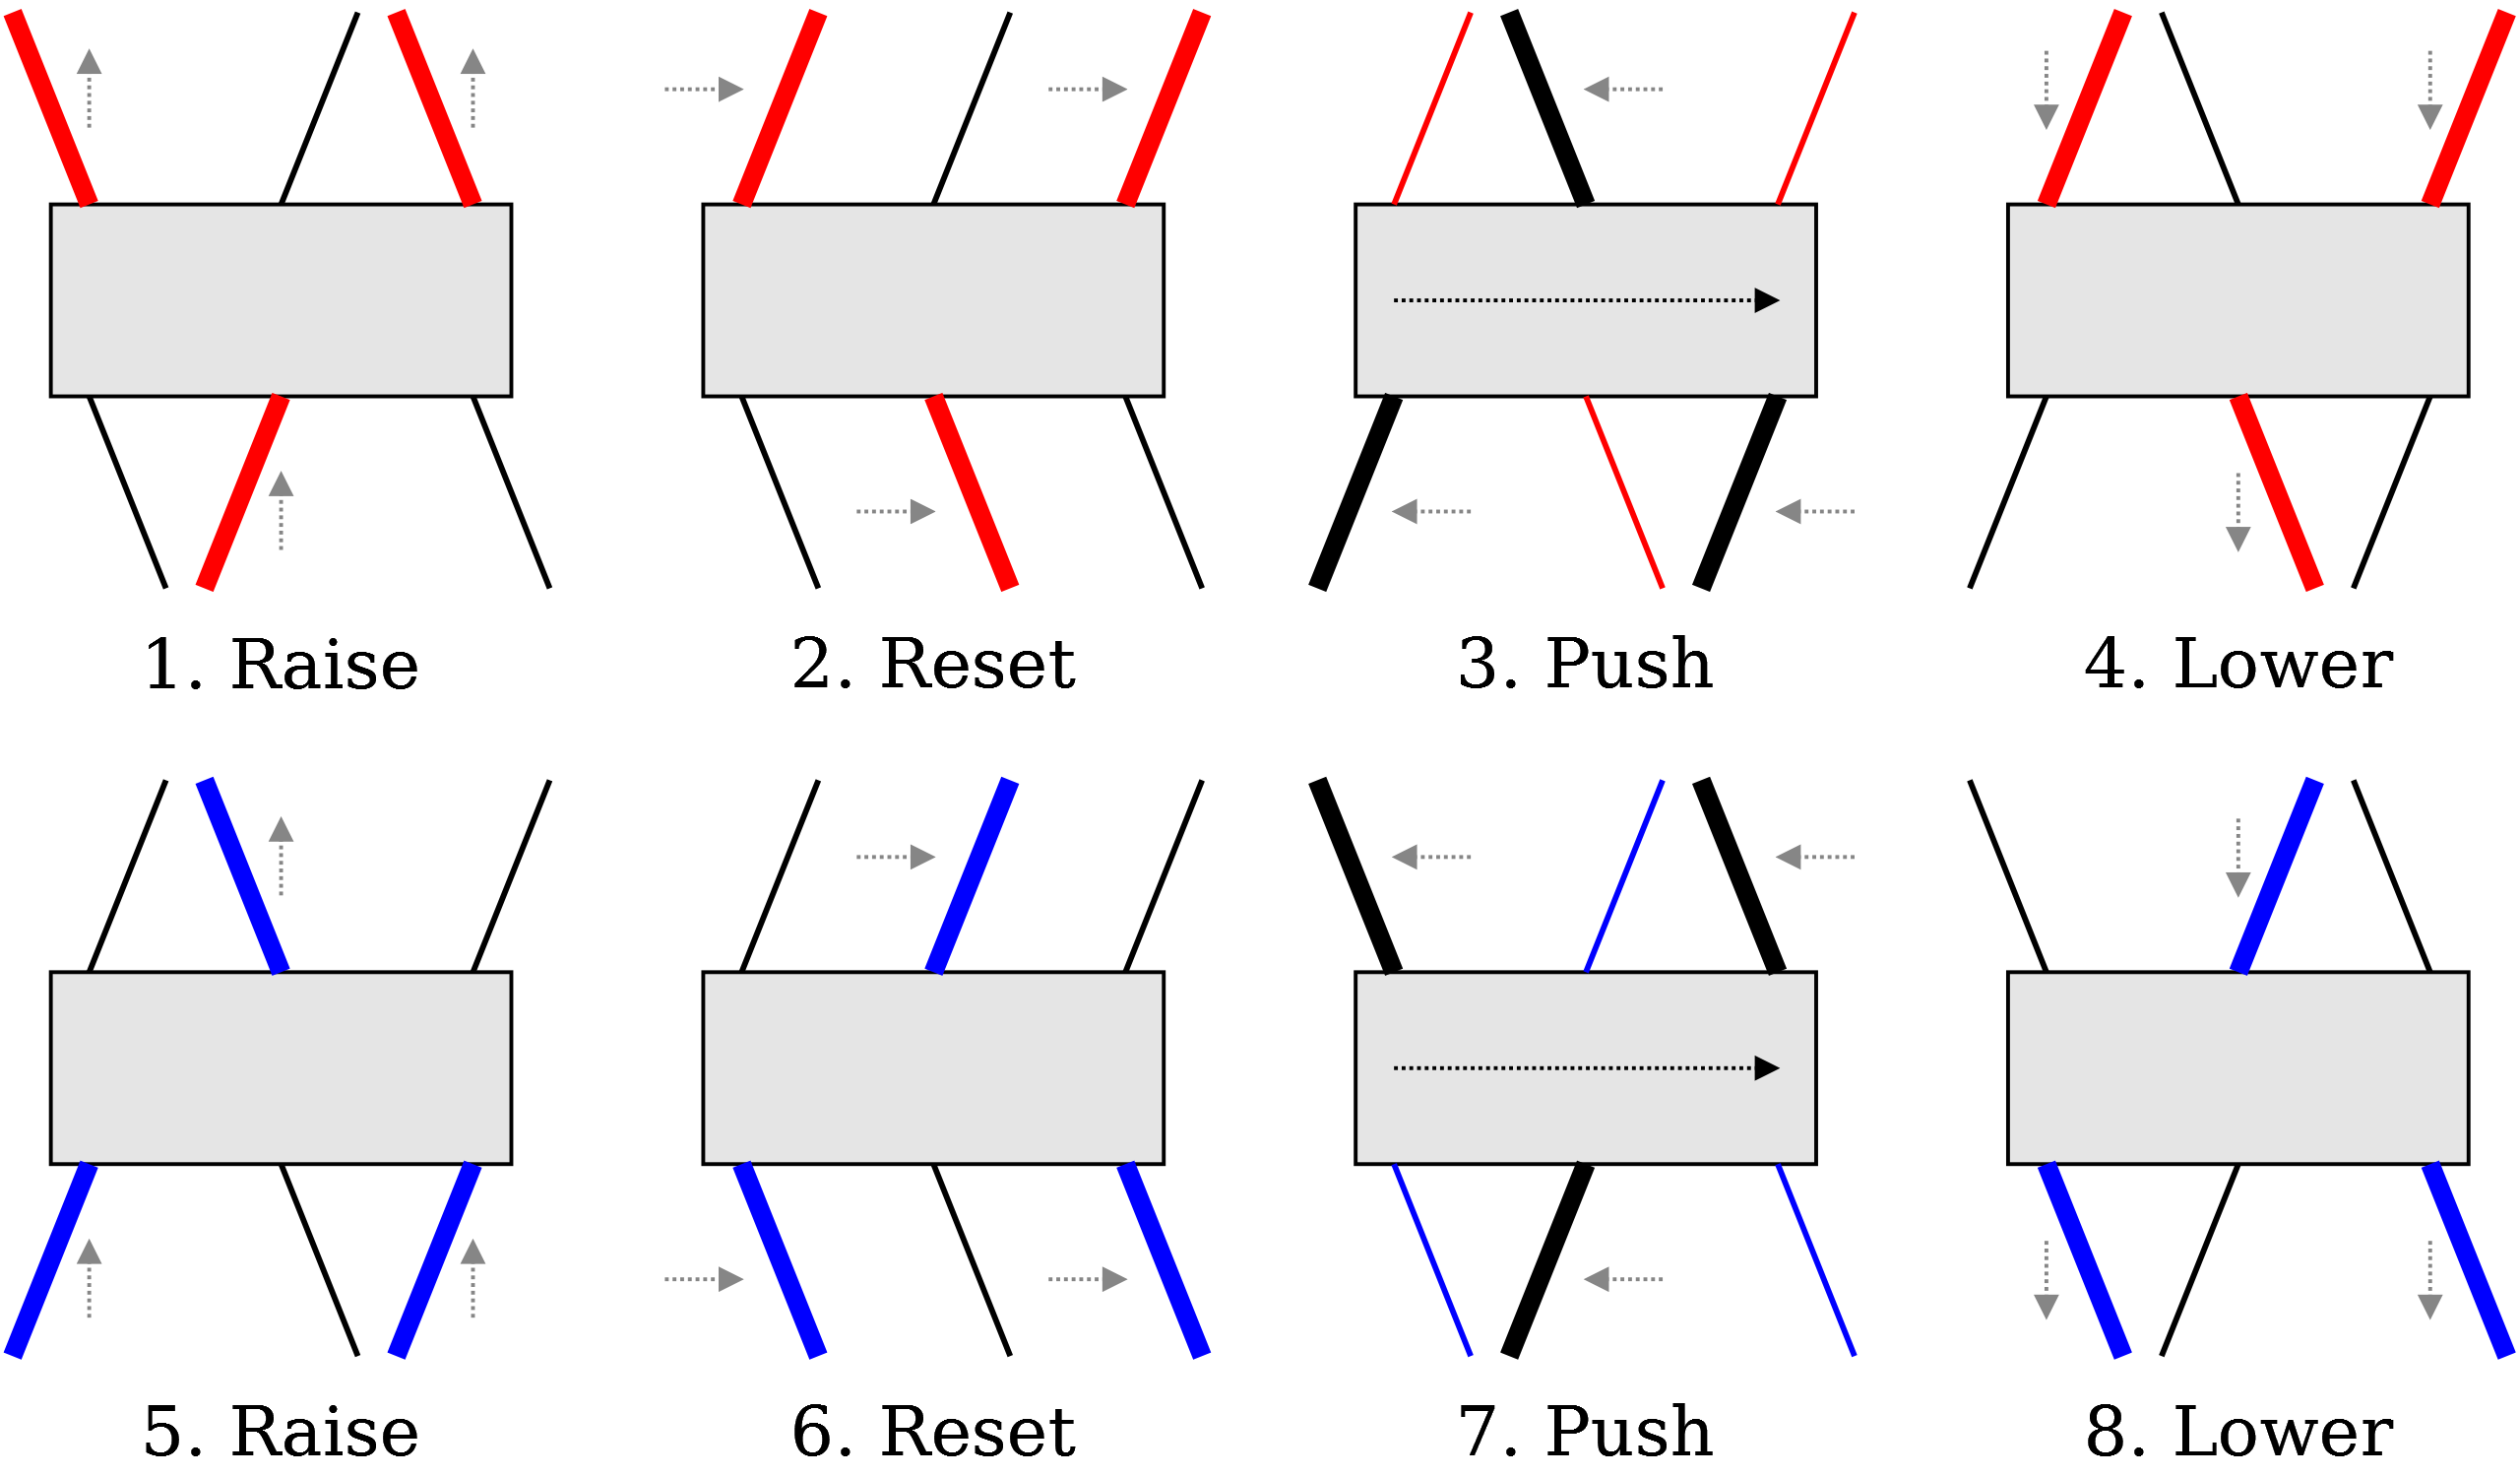
\includegraphics[width=15cm]{tripod.png}
    \vspace{1em}
    \hrule
    \vspace{1em}
    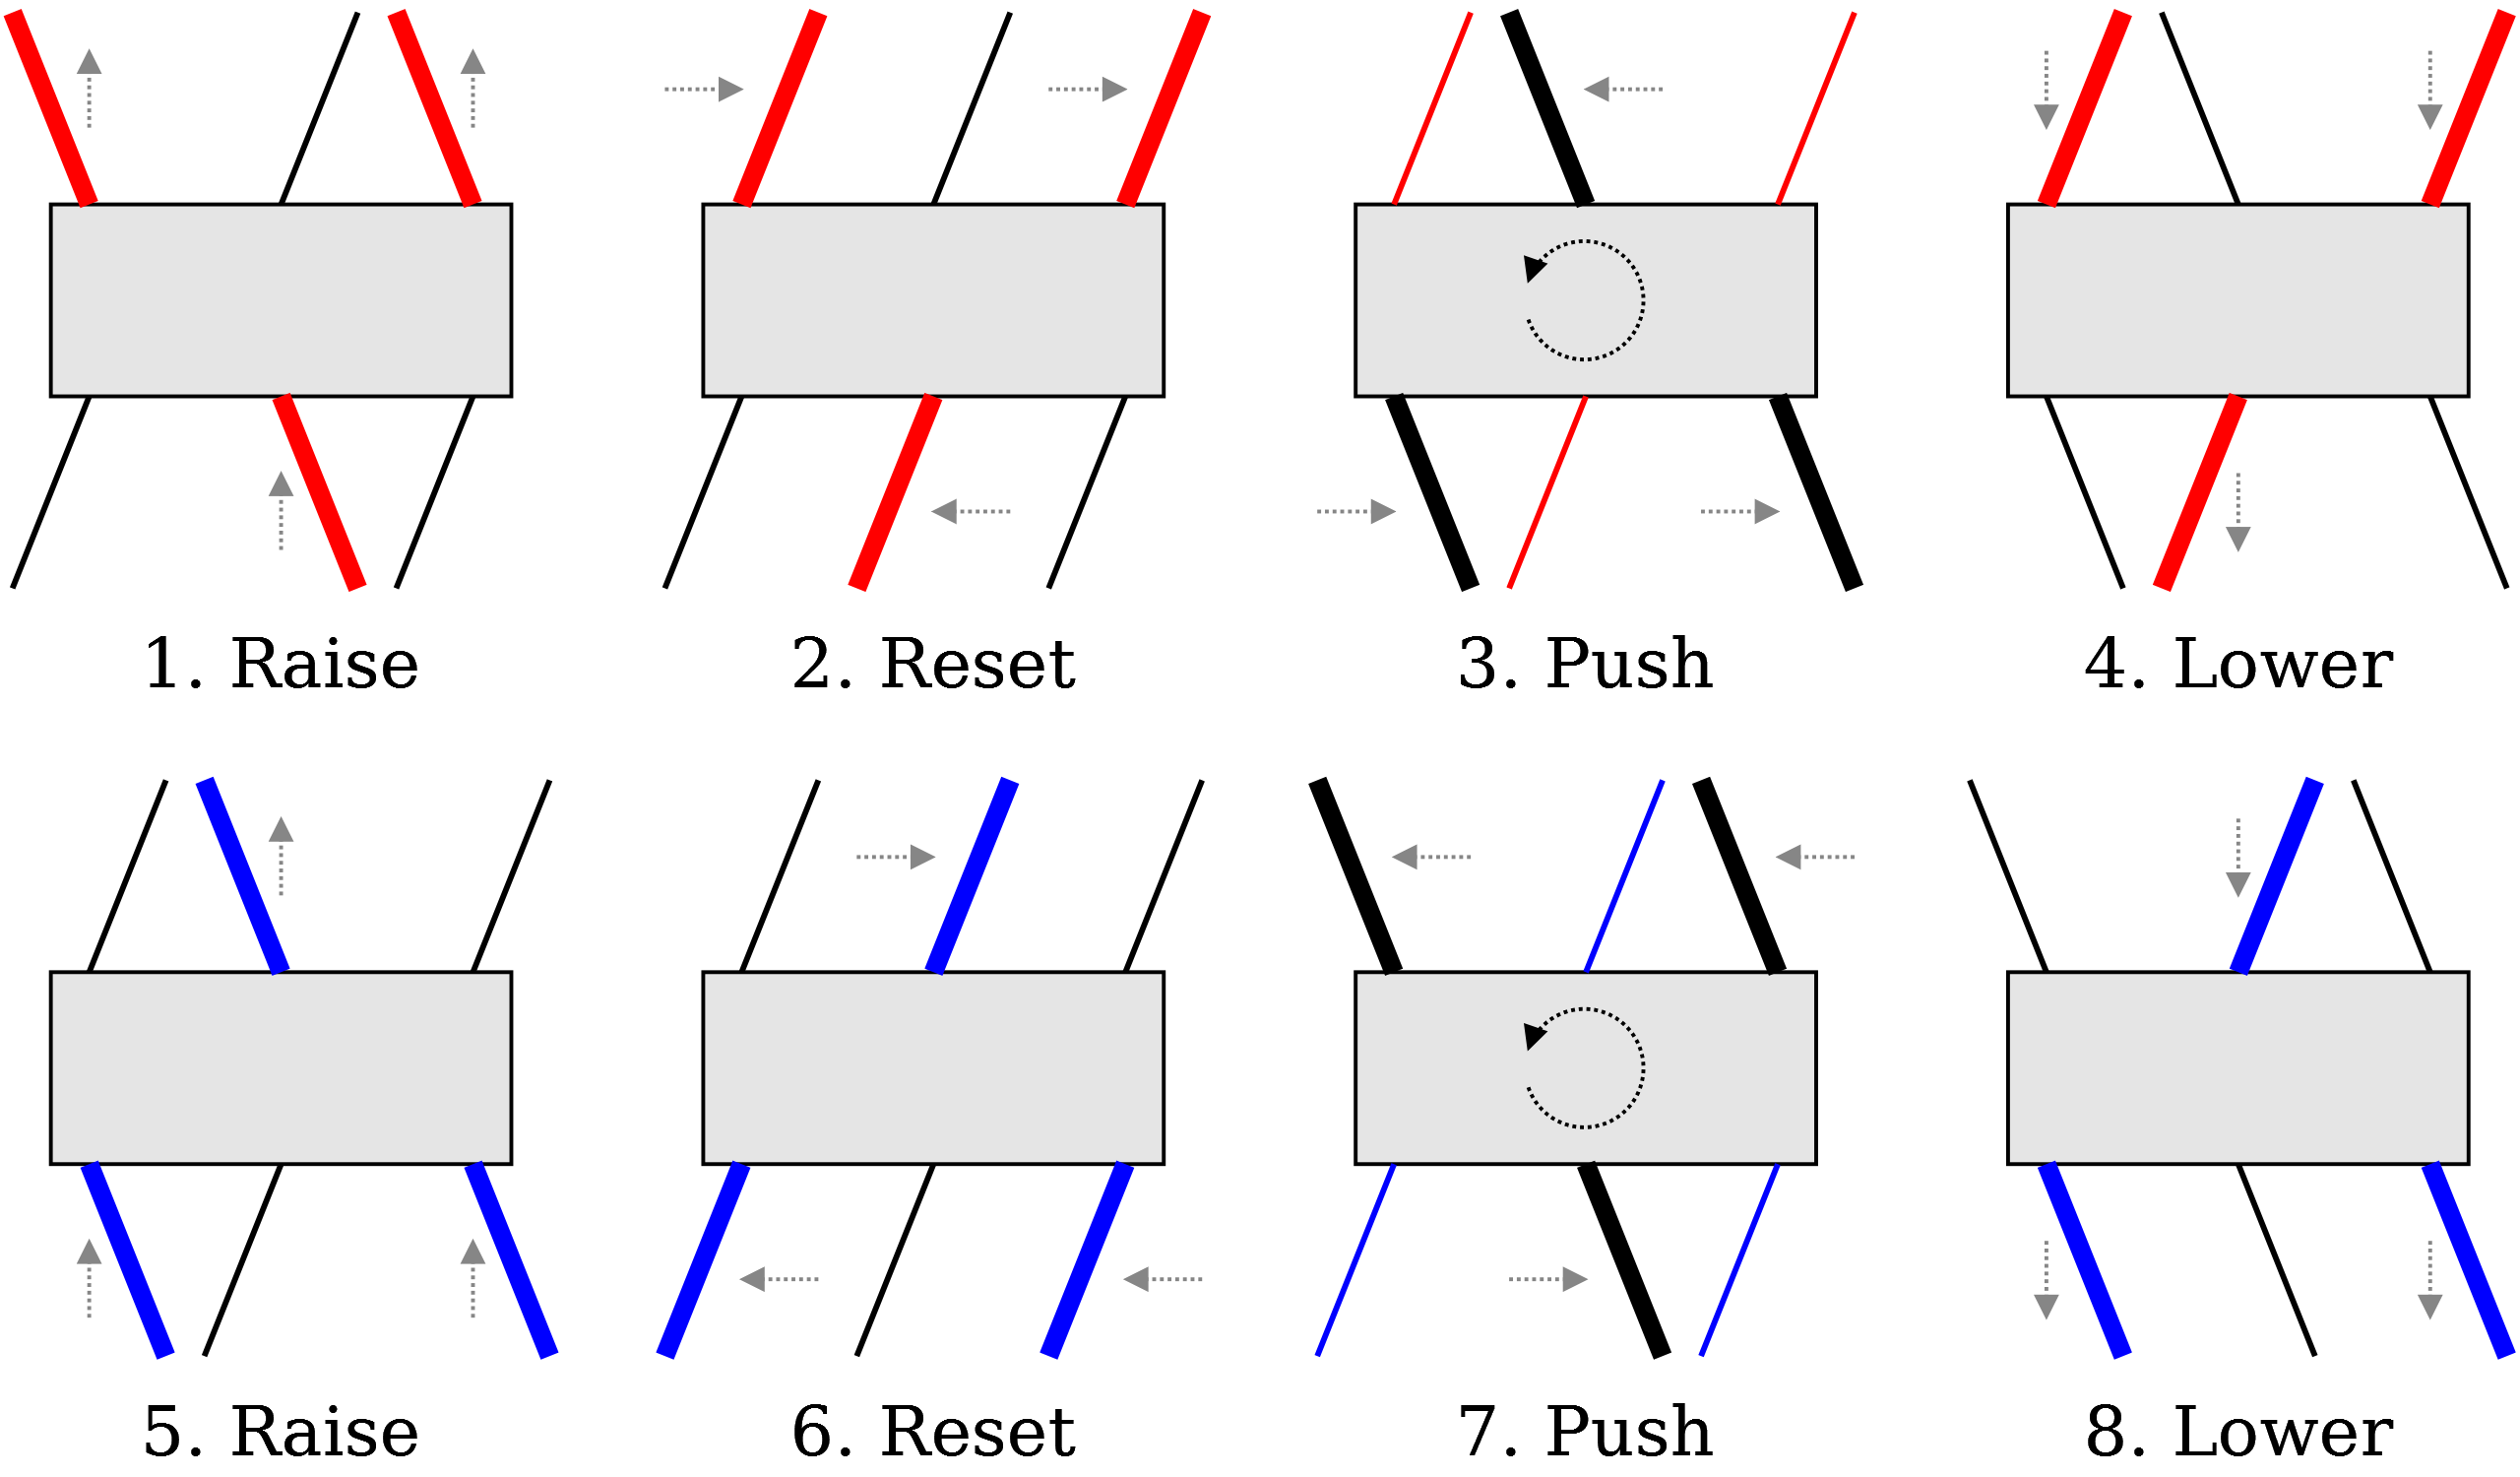
\includegraphics[width=15cm]{tripod2.png}
    \caption{Two diagrams showing a top-down view at each stage of the tripod walk gait for forward and rotational motions. Limbs coloured red and blue indicate the \emph{upper} group, while black limbs indicate the \emph{lower} group. An emboldened line along with an arrow indicates movement for that particular limb at that stage.}
    \label{fig:tripod_gait_forward}
\end{figure}


\subsection{Gamepad Controller}

Manual locomotion control was implemented using a custom \texttt{gamepad\_controller} node powered by the \texttt{joy} package, a standard package for a interfacing with joysticks and gamepads in a device-agnostic way through topics. A gamepad consists of a number of physical controls that a user can manipulate, such as buttons and analogue sticks. Buttons provide a digital output (i.e., currently pressed or not pressed) whereas analogue sticks provide a pair of coordinates ranging from $(-1, -1)$ to $(1, 1)$ depending on their position. While the \texttt{joy} package provides generic joystick access, the \emph{Microsoft Xbox 360 Controller} was targeted specifically---shown in \autoref{fig:xbox_360}.

\begin{figure}[!h]
	\centering
	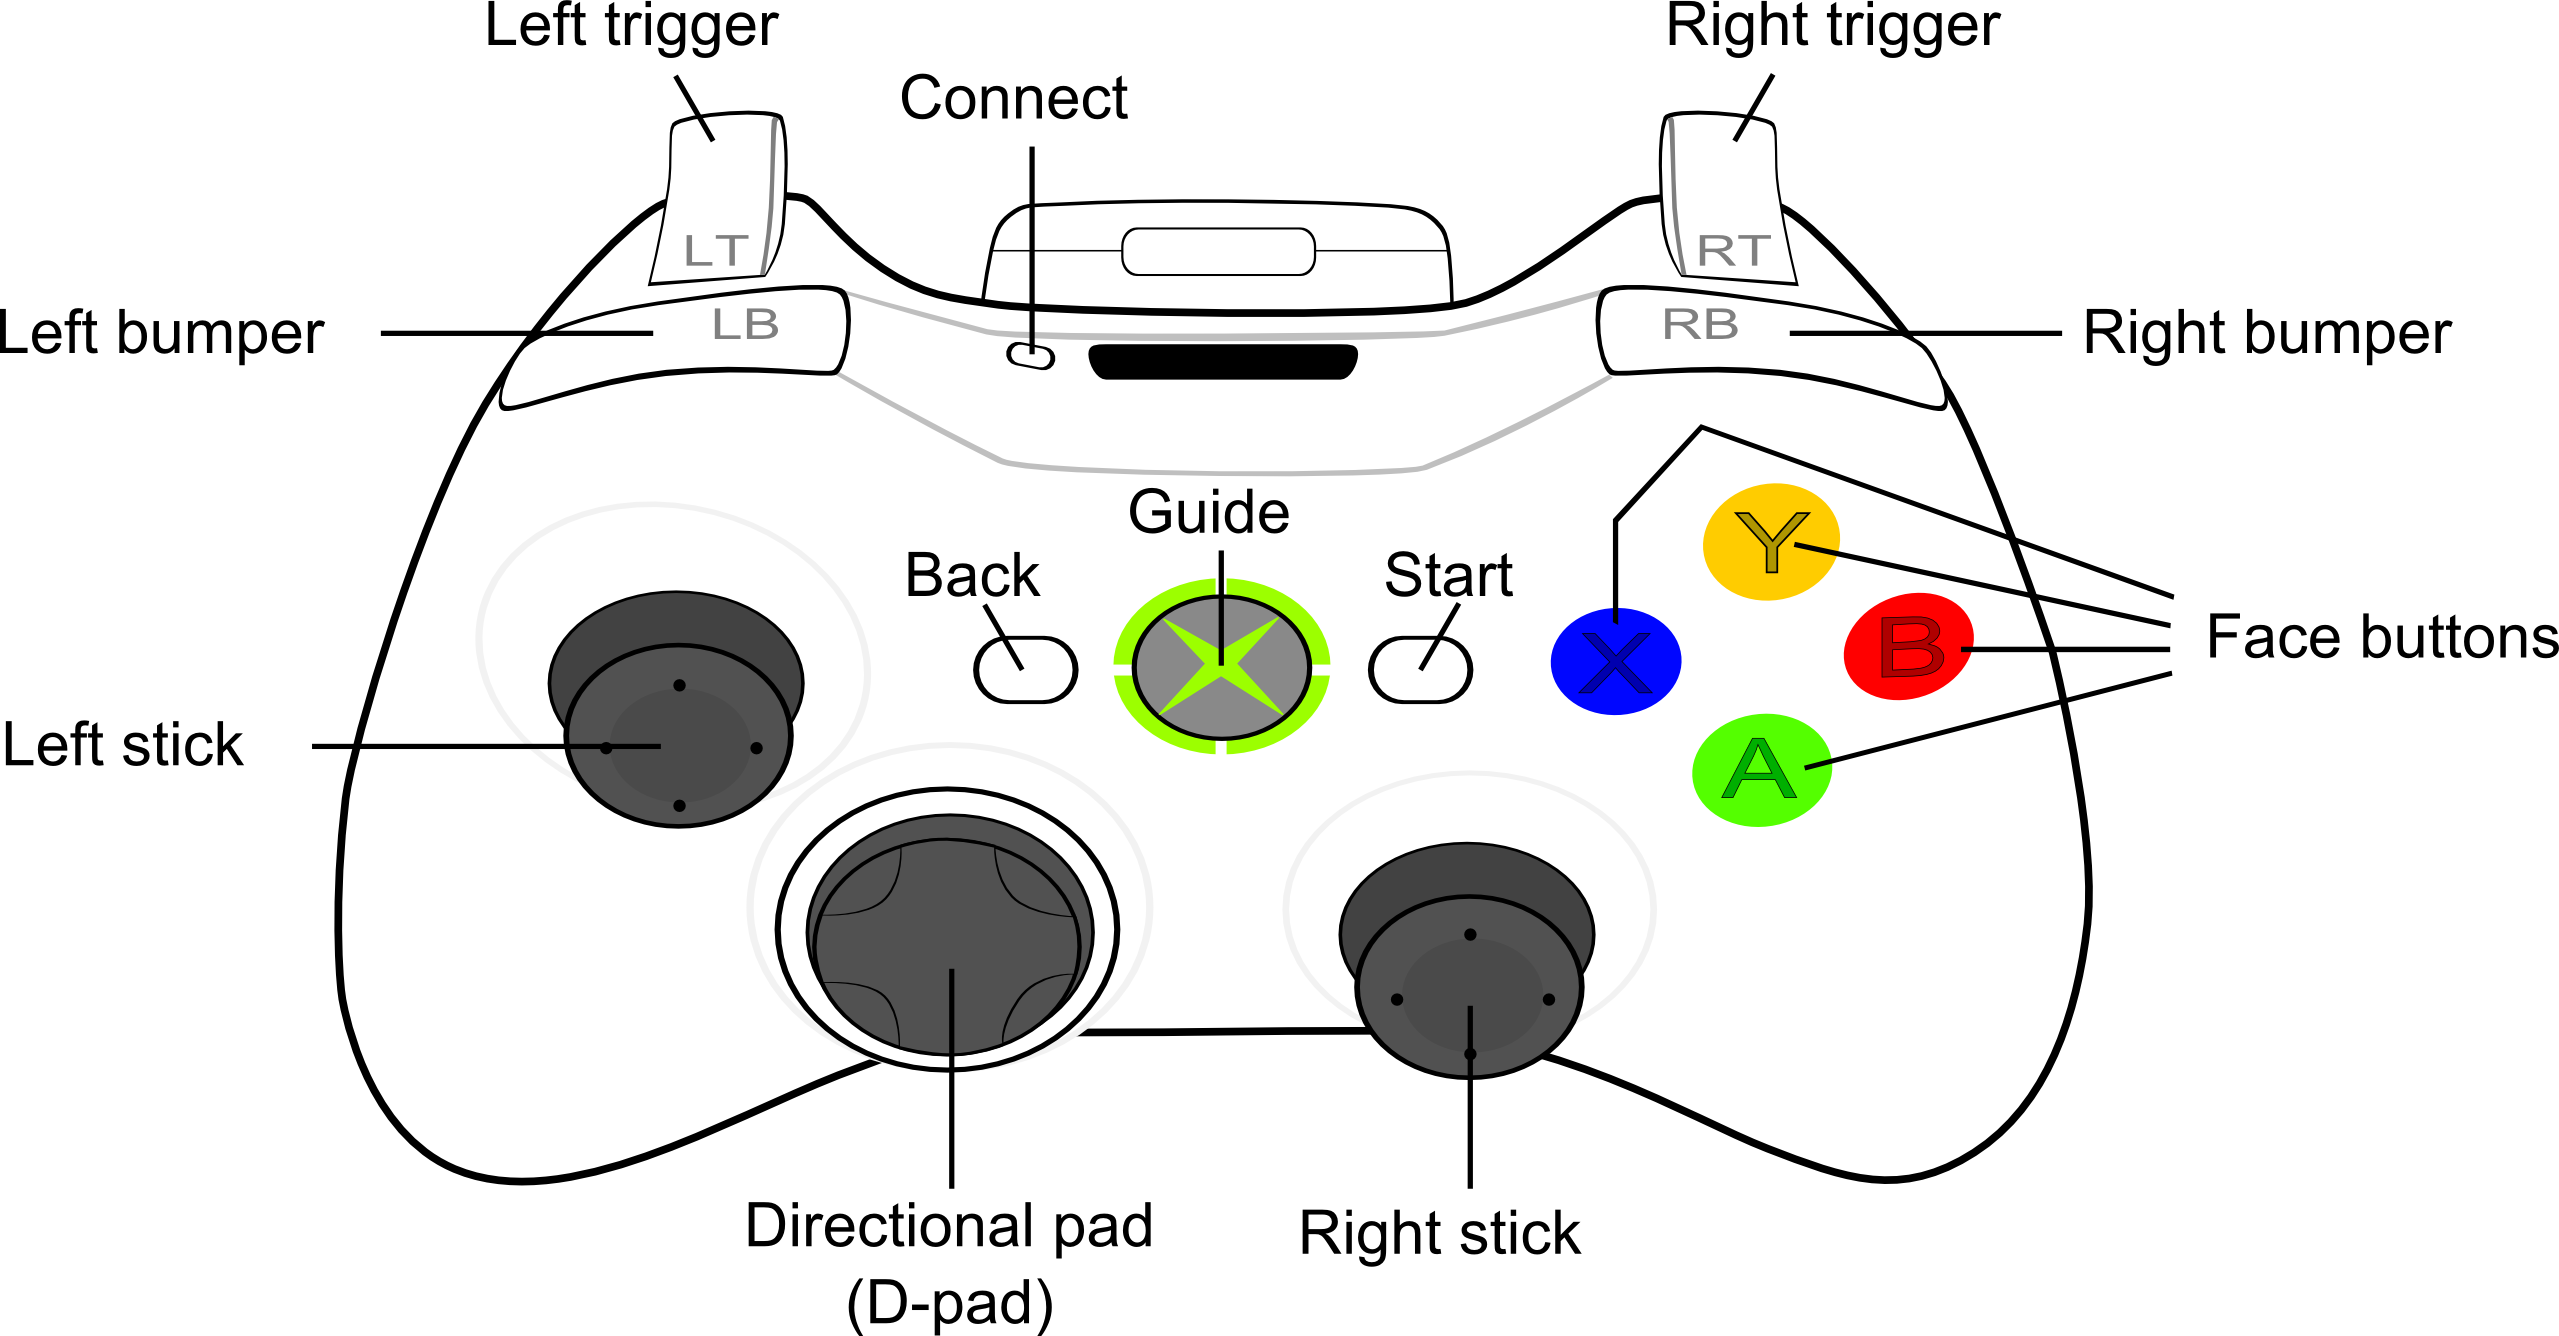
\includegraphics[width=12cm]{360.png}
	\caption{A diagram showing the layout of the Microsoft Xbox 360 Controller \cite{360_controller}. In the case of this control system, the left and right analogue sticks are used to input linear and angular motions respectively.}.
	\label{fig:xbox_360}
\end{figure}

The \texttt{joy} package contains one node named \texttt{joy\_node}. This node parses joystick input data, converts that data into standard \texttt{Joy} messages, and then broadcasts it through a \texttt{joy} topic relative to itself \cite{ros_wiki_joy}. The specification for the \texttt{Joy} message can be seen in \autoref{tab:joy_msg} and some example output from the \texttt{joy} topic can be seen in \autoref{fig:joy_example}. Additionally, \texttt{joy\_node} accepts a \texttt{dev} parameter which specifies where it should read joystick data from. If no parameter is set, the node will read data from \texttt{/dev/input/js0} which is the first controller connected to the system. 

\begin{table}[!h]
	\centering
	\begin{tabular}{ r r p{10cm} }
		\toprule
		\textbf{Name} & \textbf{Type} & \textbf{Description} \\
		\midrule

		\texttt{axes} & 
		\texttt{float32[]} &
		An array of floating point numbers indicating the current position of each axes on the controller, ranging from -1 to 1. An analogue stick like on the controller shown in \autoref{fig:xbox_360} will consist of two axes, one for the X position and the other for the Y position. \\
		\hline
		\texttt{buttons} & 
		\texttt{int32[]} & 
		An array of integers indicating the state of each button on the controller. A value of 1 indicates that the button is currently pressed, while a value of 0 indicates the opposite. \\
		\bottomrule
	\end{tabular}
	\caption{The specification for the \texttt{Joy} message as used by the \texttt{joy\_node} and \texttt{gamepad\_controller} nodes. The message also contains a \texttt{header} field but is omitted for brevity.}
	\label{tab:joy_msg}
\end{table}

\begin{figure}[!h]
	\centering
	\begin{lstlisting}
	axes:    [0.0, 0.0, 1.0, 0.0, 0.0, 1.0, 0.0, 0.0]
	buttons: [1, 0, 0, 0, 0, 0, 0, 0, 0, 0, 0]
	---
	axes:    [-1.0, 0.0, 1.0, 0.0, 0.0, 1.0, 0.0, 0.0]
	buttons: [0, 0, 0, 0, 0, 0, 0, 0, 0, 0, 0]
	---
	axes:    [0.0, 0.0, 1.0, 0.5, 0.0, 1.0, 0.0, 0.0]
	buttons: [0, 0, 0, 0, 0, 0, 0, 0, 0, 0, 0]
	\end{lstlisting}
	\caption{Some example output from the \texttt{joy} topic as provided by the \texttt{rostopic} utility. The message header has been omitted for brevity. The first message shows all axes it rest while the \emph{A} button on the controller is pressed. The second message shows the left analogue stick pushed all the way to the left with no buttons pressed. The third message shows the right analogue stick pushed halfway upwards with no buttons pressed.}
	\label{fig:joy_example}
\end{figure}

The implemented \texttt{gamepad\_controller} node listens on this \texttt{joy} topic for any controller movements. Once received, the node will send a \texttt{Twist} message to the \texttt{/cmd\_vel} topic as required by the locomotion controller. The \emph{y axis} of the left analogue, at index 1 in the axes array, is used stick for linear motion and the \emph{x axis} of the right analogue stick, in index 3 in the axes array, is used for angular motion. A ``deadzone'' had to be set on any axis movements as the analogue sticks on the controller tend not to center exactly on a $(0, 0)$ value, causing the robot to move even if the user was not touching them in any way. Instead, movement commands will only be sent if either of the axes is moved by at least one quarter of the range---i.e., $|x| \geq 0.25$.

%%%%%%%%%%%%%%%%%%%%%%%%%%%%%%%%%%%%%%%%%%%%%%%%%%%%%%%%%%%%%%%%%%%%%%%%%%%%%%%%%%%%%%%%%%%%%%%%%%%%

\section{Sensing}

The sensing subsystem was implemented as a \texttt{hexapod\_sensing} package. This subsystem provides the control system with the positional and environmental information that is necessary to facilitate autonomous navigation through the use of the RGB-D camera. Community provided packages were used to implement both components of this subsystem and, accordingly, only the general operations and interfaces they provide will be detailed. These packages provide state-of-the-art functionality through an abstracted interface, allowing us to deal with with the overall goals rather than the complex inner-workings of any one component.

\subsection{Visual Odometry}

Odometry was provided by the \texttt{visual\_odometry} node included in the \texttt{ccny\_rgbd} package, a package provided by \emph{City University of New York} \cite{ccny_rgbd}. This node is used to estimate any motions of the camera on-board the robot such that its position can be determined relative to its starting position. A combination of the colour and depth imagery from the camera is used to achieve this. It should be noted that the \texttt{ccny\_rgbd} package additionally provides a suite of nodes for performing further processing on the imagery---e.g., scaling, registartion, warping, etc---but we chose not to use these nodes as they target \emph{OpenNI} rather than \emph{OpenNI2}. While an attempt to use the nodes was made, they tended to result in a nosier image than using the feed directly from the \texttt{openni2\_camera} node. Furthermore, the \texttt{openni2\_camera} node already provides the registration functionality---which aligns the depth and colour images---as required by the \texttt{visual\_odometry} node.

The \texttt{visual\_odometry} node expects colour and depth imagery as a stream of \texttt{Image} messages on the \texttt{/rgbd/rgb} and \texttt{/rgbd/depth} topics respectively \cite{ccny_rgbd_vo}. These are the topics published by the \texttt{ccny\_rgbd} processing nodes and thus had to be remapped to the correct topics coming from the \texttt{openni2\_camera} node, specifically \texttt{/camera/rgbd/image\_raw} and \texttt{/camera/depth\_registered/image\_raw}. This remapping was done through the use of \emph{roslaunch} as will be explained in \autoref{sec:integration}.

When running, the node publishes a \emph{tf} transform between \texttt{odom} and \texttt{base\_link} which gives an estimated position of the robot relative to its starting position. An additional node from the \emph{tf} package, specifically a \texttt{static\_transform\_publisher}, is used to publish a transform between \texttt{map} and \texttt{odom} in order to complete the transform tree. As no localisation based on mapping can be performed, we assume that these frames are in identical positions relative to each other. The resulting transform tree was shown in \autoref{fig:tf_tree}. This can then be used by the mapping and navigational systems as required.

\subsection{Environment Mapping}

Mapping facilities where provided by the \texttt{octomap\_server} node included in the \texttt{octomap\_mapping} package, developed by the \emph{University of Freiburg} \cite{ros_wiki_octomap}. This acts as a wrapper for the \emph{OctoMap} library, written in C++, which supplies a number of algorithms and data structures necessary for 3D environment mapping \cite{octomap, hornung13auro}. The \texttt{octomap\_map} node encapsulates the complexities of this library and provides access to it through standard ROS topics and services. By supplying the node with a position estimate and depth imagery from an RGB-D camera, a dynamic 3D occupancy map can be generated of the environment surrounding the robot. Any obstacles that are placed in front of the robot will cause the map to update to reflect the change in environment. This map can then be compressed into a 2D occupancy map as required by the navigational system.

This particular mapping solution was chosen as it was the only one that could be found intended for RGB-D cameras from the ground up. Other solutions tended to require expensive laser scanners to produce an interpretation of the environment. While it is possible to emulate the output of a laser scanner using an RGB-D camera, the resulting maps were not of as high quality as those produced by the \texttt{octomap\_mapping} package. 

In particular, the \texttt{octomap\_server} node expects \texttt{PointCloud2} messages on a \texttt{cloud\_in} topic \cite{ros_wiki_octomap_server}. This topic is remapped through \emph{roslaunch} to the point cloud published by the camera driver which is located on the \texttt{/camera/depth/points} topic. A \emph{tf} transform between the sensor frame noted in the \texttt{PointCloud2} message---\texttt{camera\_depth\_frame} in this case---and the static \texttt{map} frame is also necessary. These transforms are provided by the visual odometry system and the full transform tree can be seen in \autoref{fig:tf_tree}.

While running, the node publishes \texttt{OctomapBinary} messages to an \texttt{octomap\_binary} topic \cite{ros_wiki_octomap_server}. These messages can be used to visualise the resulting interpretation of the environment in 3D through \emph{RViz}, an example of which was shown in \autoref{fig:rviz}. The node also publishes \texttt{OccupancyGrid} messages to a \texttt{projected\_map} topic providing a 2D interpretation of the environment by flattening the generated 3D map \cite{ros_wiki_octomap_server}. To elaborate further, maps are represented as an \emph{occupancy grid} in that the map is split into a number of cells where each cell is defined as occupied, unoccupied, or unknown. An \texttt{OccupancyGrid} messages represents the environment in this manner using a two-dimensional array of integers \cite{ros_api_og_msg}. These messages are then supplied to the navigational system for obstacle avoidance and path planning.

%%%%%%%%%%%%%%%%%%%%%%%%%%%%%%%%%%%%%%%%%%%%%%%%%%%%%%%%%%%%%%%%%%%%%%%%%%%%%%%%%%%%%%%%%%%%%%%%%%%%

\section{Navigation}

To implement the autonomous navigation system, the standard \texttt{navigation} package was used. This package actually encompasses a number of other packages implementing a full suite of facilities necessary for performing autonomous navigation tasks, and is distributed with ROS as standard \cite{ros_wiki_nav}. The \texttt{move\_base} package, in particular, which contains a similarly named \texttt{move\_base} node which provides a single simplified access point to these facilities \cite{ros_wiki_nav_base}. By providing this node with access to a map, positional information, movement control, and a target goal, as well as some general configuration, it will apply the suite in such a way that the robot can navigate to the target goal autonomously while avoiding any obstacles in the way. It should be noted that the \texttt{navigation} package is intended for wheeled robots, however our abstracted walking system allows us to use it with this hexapod-style robot as required.

The \texttt{move\_base} node requires a number of inputs and outputs to function correctly. A \emph{tf} transform must be published linking the \texttt{map} frame to the \texttt{base\_link} frame such that the robot's position can be known throughout the movement process. A map must be published as \texttt{OccupancyGrid} messages on the \texttt{map} topic, allowing the navigation system to generate a movement path accordingly. Finally, a topic that can be used to control the robots velocity via \texttt{Twist} messages must be available. All of the subsystems that have been detailed up until this point provide these input and outputs, plugging directly into the \texttt{move\_base} node as required. A number of parameters must also be set for the \texttt{move\_base} node to function correctly. These parameters detail the shape of the robot, maximum velocities, tolerances for reach the goal and so on.

While running, the \texttt{move\_base} node listens for a \texttt{PoseStamped} message on the \texttt{goal} topic \cite{ros_wiki_nav_base}. This message contains a header along with another \texttt{Pose} message, which simply contains a position in space---in $x$, $y$, $z$ components---along with a rotation \cite{ros_api_posestamped}. Once a message has been received, the node will carry out the path planning procedure resulting in a path that can be followed to get to that position, avoiding any obstructions in the way. \emph{rviz} can be used to specify this goal, simplifying the targeting process for any operator. 

Once the path has been planned, the node will then provide the necessary \texttt{Twist} messages to our custom \texttt{walk\_controller} node, thus moving the robot to the requested location. This operates on a feedback loop, whereby the node constantly checks the reported position of the robot versus where it should be on the path, adjusting the movements commands sent as necessary. Additionally, if any new obstacles appear on the map, the path planner will rerun such that the robot can avoid the obstacle. Should the robot get stuck---e.g., it does not progress along the path after a number of seconds--- then the \texttt{move\_base} node attempts a number of recovery behaviours. These generally comprise of rotating the robot on the spot such that the mapping system can re-evaluate the surrounding environment.

%%%%%%%%%%%%%%%%%%%%%%%%%%%%%%%%%%%%%%%%%%%%%%%%%%%%%%%%%%%%%%%%%%%%%%%%%%%%%%%%%%%%%%%%%%%%%%%%%%%%

\section{Integration}
\label{sec:integration}

Finally, this last implementation section will detail the specifics of how the subsystems were integrated to create the complete robot control system, as well as how an operator interacts with the system to issue commands. Integration is made fairly trivial through the use of \emph{roslaunch} and, as such, this section is rather short.

\subsection{Running the Robot Control System}

While it is possible to start each node separately, a number of \emph{roslaunch} launch files were created to assist in this process. The result is a means for starting the robot control system in its entirety with one terminal command only. This implementation process for this was fairly trivial as \emph{roslaunch} provides great flexibility through its launch files.

Launch files were first created for each subsystem. These would start the nodes necessary for the subsystem, supplying any parameters and topic remappings as required---the specifics of which have been detailed in the previous sections. Then, a master launch file that includes the launch files for each subsystem was created. By running this launch file with \emph{roslaunch}, the ROS master will be started along with all of the control system nodes.

\subsection{User Visualisation and Commands}

A \emph{rviz} configuration was created to visualise topic outputs from the control system at run-time as is shown in \autoref{fig:rviz}. This configuration allows an operator to see the raw imagery from the RGB-D sensor along with a 3D view of environment around the robot. Additionally, positional and path planning data can be seen as the robot moves around the environment. \emph{rviz} also provides a facility for setting navigational goals by simply clicking on the 3D environment.